\documentclass[../final_report_main.tex]{subfiles}
\begin{document}
%Handy Shortcut Macros
\newcommand\mX[1]{\multicolumn{1}{X}{#1}}
\newcommand\mcc[1]{\multicolumn{2}{c}{#1}}
\newcommand\mcl[1]{\multicolumn{2}{l}{#1}}
\begin{table}[H]
\centering
\begin{tabular}{ccccc}
\toprule
{Angles} & \multicolumn{4}{c}{Distance}\\\cmidrule{2-5}
& \mcc{\textbf{15 cm}}
& \mcc{\textbf{30 cm}}\\
\cmidrule{2-3} \cmidrule{4-5}
& {(+)}  & {(-)} & {(+)} & {(-)} \\
\midrule
12 & 0.10 & 1.82 & 0.10 & 1.46\\\hline
10 & 4.53 & 6.61 & 1.02 & 3.02\\\hline
8 & 17.66 & 16.09 & 1.84 & 5.63\\\hline
6 & 31.69 & 30.57 & 4.46 & 7.53\\\hline
5 & 37.70 & 33.87 & 5.16 & 9.26\\\hline
4 & 37.08 & 30.81 & 8.32 & 9.41\\\hline
3 & 40.90 & 37.20 & 9.13 & 9.77\\\hline
2 & 43.21 & 40.98 & 9.67 & 10.23\\\hline
1 & 42.67 & 40.22 & 10.02 & 10.10\\\hline
0 & 41.33 & 41.33 & 11.47 & 11.47\\\hline
\bottomrule
\end{tabular}
\caption{Measured coincidence data (counts per second) at varied offset angles
(degrees) and distances. In correspondance with model 1.}
\label{table:model1_table}
\end{table}
%Table 2 of Overlapping Area Data
\begin{table}[H]
\centering
\begin{tabular}{ccccc}
\toprule
{Angles} & \multicolumn{4}{c}{Distance}\\\cmidrule{2-5}
& \mcc{\textbf{15 cm}}
& \mcc{\textbf{30 cm}}\\
\cmidrule{2-3} \cmidrule{4-5}
& {(+)}  & {(-)} & {(+)} & {(-)} \\
\midrule
12 & 27.79 & 27.79 & 6.70 & 6.70\\\hline
10 & 31.96 & 31.96 & 13.01 & 13.01\\\hline
8 & 39.26 & 39.26 & 25.87 & 25.87\\\hline
6 & 40.41 & 40.41 & 28.05 & 28.05\\\hline
5 & 42.53 & 42.53 & 32.12 & 32.12\\\hline
4 & 44.63 & 44.63 & 36.26 & 36.26\\\hline
3 & 46.70 & 46.70 & 40.25 & 40.25\\\hline
2 & 48.68 & 48.68 & 44.64 & 44.64\\\hline
1 & 50.25 & 50.25 & 48.68 & 48.68\\\hline
0 & 50.27 & 50.27 & 50.27 & 50.27\\\hline
\bottomrule
\end{tabular}
\caption{Measured overlapping area ($m^{2}$) at varied offset angles
(degrees) and distances. In correspondance with model 2.}
\label{table:model2_table}
\end{table}
%Figure 1
\begin{figure}[H]
    \centering
    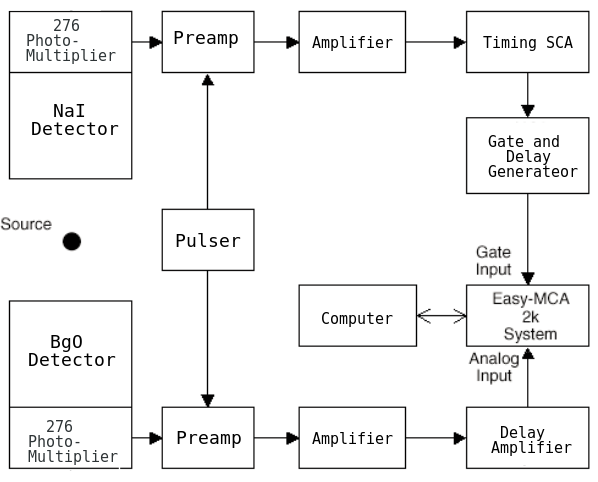
\includegraphics[width=.45\textwidth]{Figures/gamma_coin_circuitry.png}
    \caption{Circuitry behind the detectors used to measure gamma coincidence
    (Inspired by \cite{Experiment_Set_Up:1}).}
    \label{figure:circuitry}
\end{figure}
%Figure 2
\begin{figure}[H]
     \centering
     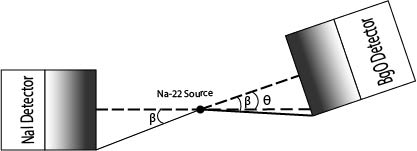
\includegraphics[width=.45\textwidth]{Figures/detector_set_up.jpg}
     \caption{Set up of angular variation between the two detectors and the
     \textsuperscript{22}Na source (inspired by \cite{Experiment_Set_Up:2}).}
     \label{figure:set_up}
\end{figure}
%Figure 3
\begin{figure}[H]
    \centering
    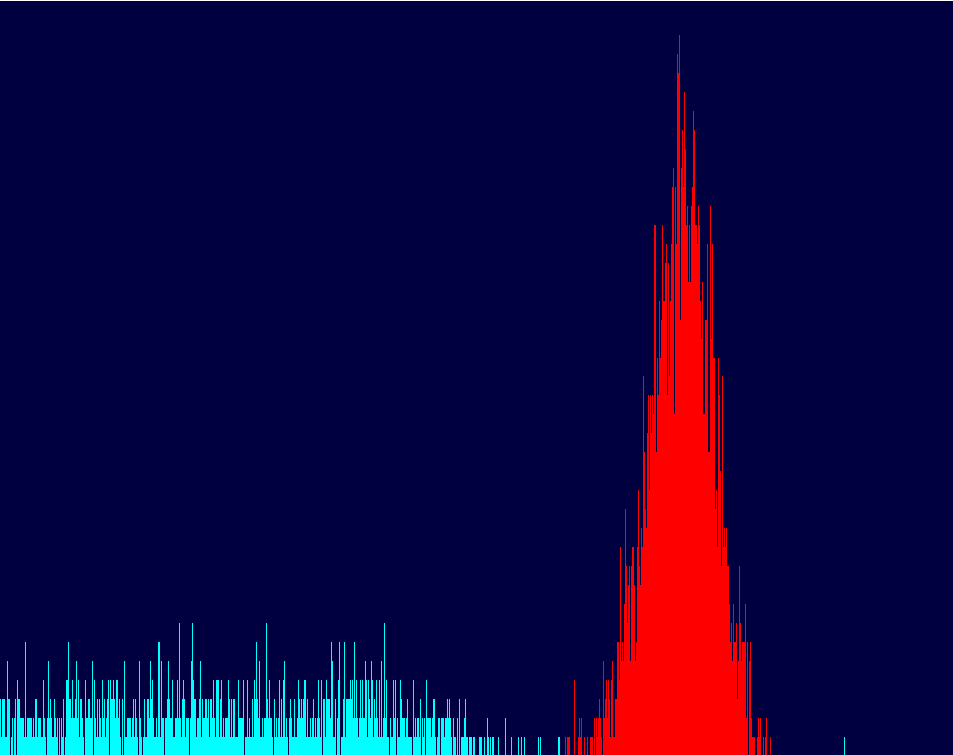
\includegraphics[width=0.9\linewidth]{Figures/sample_spectrum.png}
    \caption{Spectrum produced with the detectors 15 cm and 0 degrees offset
    from the source. Peak highlighted was integrated for count rate.}
    \label{figure:spectrum}
\end{figure}
%Figure 4, 5, & 6
\begin{figure}[H]
    \centering
    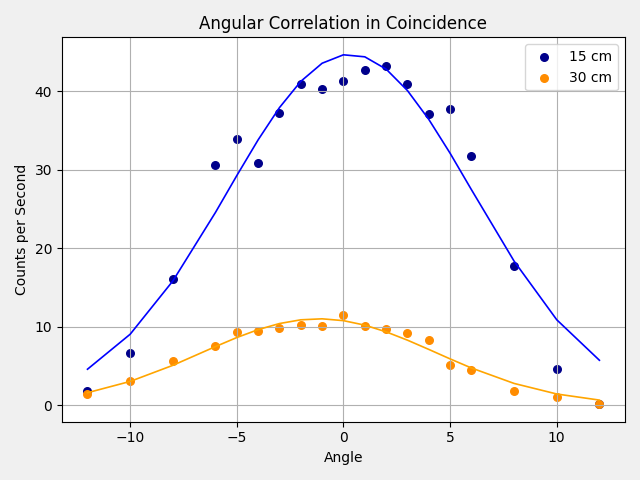
\includegraphics[width=0.45\textwidth]{Figures/coincidence_gauss_fit.png}
    \caption{Table \ref{table:model1_table} visualized and fitted with a Gaussian
    function.}
    \label{figure:model1_graph}
    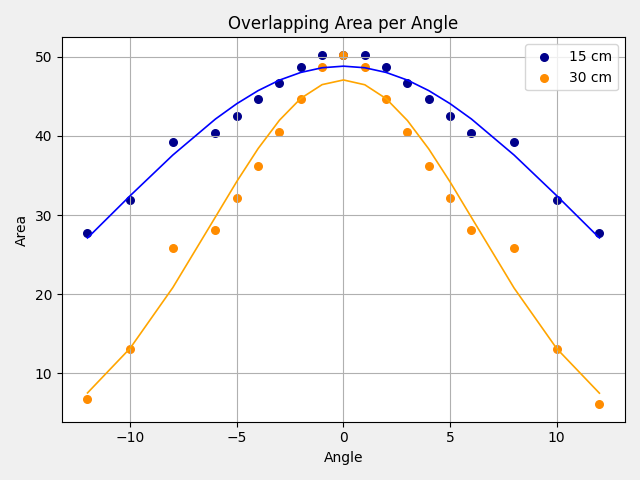
\includegraphics[width=0.45\textwidth]{Figures/overlapping_area_gauss_fit.png}
    \caption{Table \ref{table:model2_table} visualized and fitted with a Gaussian
    function.}
    \label{figure:model2_graph}
    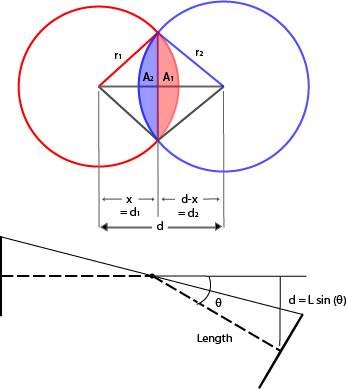
\includegraphics[width=0.45\textwidth]{Figures/geometry.jpg}
    \caption{Set up of the geometry used to derive the correlation between
    overlapping area and angular offset (inspired by \cite{Geometry}).}
    \label{figure:geometry}
\end{figure}
\end{document}
